\section{Theorie}
\label{sec:Theorie}

\subsection{Funktionsweise des Rasterkraftmikroskops}
\label{sec:Rasterkraftmikroskop}

Das Rasterkraftmikroskop basiert auf dem Hookesche Gesetz $F= -k\Delta z$, mit
der Federkonstante $k$ und der Auslenkung $\Delta z$ des Federbalkens bzw. Cantilevers.
Bei dem Cantilever handelt es sich um einen Arm, der an einer Seite fest montiert
ist und am anderen Ende frei schwingen kann (siehe Abbildung \ref{fig:AFM}).

\begin{figure}[H]
	\centering
	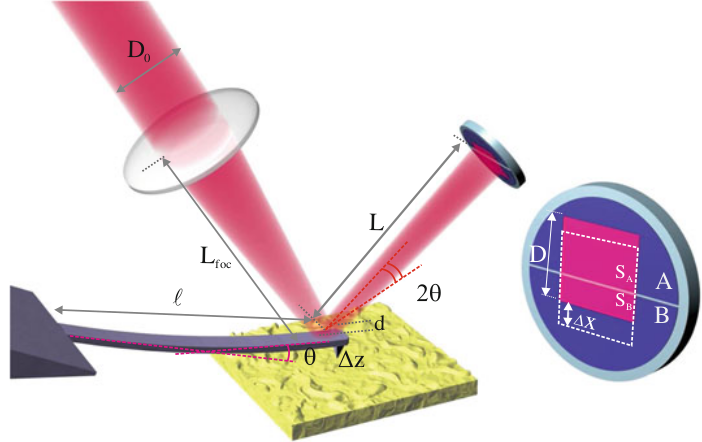
\includegraphics[width=0.63\textwidth]{Abb/AFM.png}
	\caption{Schematische Darstellung des Rasterkraftmikroskops. In gelb ist die
  Probe dargestellt. Von links ragt das Cantilever samt Messspitze auf die Probe.
  Rotes Laserlicht wird mittels einer Linse auf den Rücken des Cantilevers
  fokussiert und dort zur Photodiode reflektiert. Es handelt sich in der Abbildung
  um eine Zweisegment-Photodiode, anstelle einer in diesem Versuch verwendeten
  Viersegment-Photodiode \cite[161]{AFM}.}
	\label{fig:AFM}
\end{figure}

\noindent
An dem frei schwingendem Ende ist eine Messspitze, mit einem Radius von weniger
als $\SI{10}{\nano\meter}$. Das Cantilever sollte eine kleine Federkonstante $k$ haben,
damit diese sensibel auf Wechselwirkungen mit der Probe reagiert. Die Größenordnung
der Federkonstante $k$ lässt sich dabei folgendermaßen abschätzen: Das Gewicht
eines Atoms ist in etwa $m_{\text{At}} \approx \SI{e-25}{\kilo\gram}$ und
die typische Vibrationsfrequenz von Festkörperatomen liegt bei $\omega_{\text{vib}}
\approx\SI{e13}{\hertz}$, damit ergibt sich nach

\begin{equation}
  \omega = \sqrt{\frac{k}{m}}
  \iff
  k = \omega^2 m
  \label{eq:F1}
\end{equation}

\noindent
eine Federkonstante $k$ in der Größenordnung von $\sim\SI{10}{\newton\per\meter}$ \cite[157]{AFM}.
Ein harmonischer Oszillator wird bekanntlich nur dann zur Schwingungen angeregt,
wenn die Anregungsfrequenz $\omega_{\text{ex}}$ deutlich kleiner ist, als die
der Resonanzfrequenz $\omega_{\text{rf}}$. So sollte auch das Cantilever eine
hohe Resonanzfrequenz ($\gg \SI{10}{\kilo\hertz}$) aufweisen, welche erlaubt,
mit hohen Scan-Geschwindigkeiten zu messen. Zusätzlich wird so auch die Stabilität
vor Messverfälschungen wie externen Vibrationen gewährleistet. Damit nach Formel \ref{eq:F1}
die Resonanzfrequenz $\omega_{\text{rf}}$ klein gehalten wird, sollte das
Cantilever wenige $\mu g$ wiegen. In Abbildung \ref{fig:typen} sind vier verschiedene
Verfahren dargestellt, die es erlauben, die Cantileverauslenkung $\Delta z$ zu bestimmen.
Neben dem im Abbildung \ref{fig:AFM} gezeigten Lichtzeigerprinzip \ref{fig:typ1},
gibt es das Interferometrieprinzip \ref{fig:typ2}, den Piezoresistiven
\ref{fig:typ3} und den Piezoeletrischen Effekt \ref{fig:typ4}.


\begin{figure}[H]
\centering
	\begin{subfigure}[t]{0.24\textwidth}
	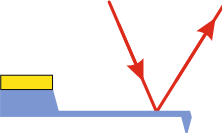
\includegraphics[width=\textwidth]{Abb/typ1.png}
  \caption{Lichtzeigerprinzip}
  \label{fig:typ1}
	\end{subfigure}
	~
	\begin{subfigure}[t]{0.22\textwidth}
	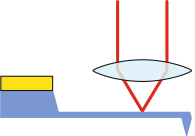
\includegraphics[width=\textwidth]{Abb/typ2.png}
  \caption{Interferometrieprinzip}
  \label{fig:typ2}
	\end{subfigure}
  ~
  \begin{subfigure}[t]{0.22\textwidth}
  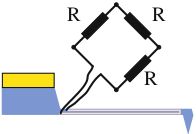
\includegraphics[width=\textwidth]{Abb/typ3.png}
  \caption{Piezoresistiver Effekt}
  \label{fig:typ3}
  \end{subfigure}
  ~
  \begin{subfigure}[t]{0.22\textwidth}
  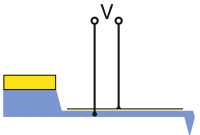
\includegraphics[width=\textwidth]{Abb/typ4.png}
  \caption{Piezoeletrischen Effekt}
  \label{fig:typ4}
  \end{subfigure}
	\caption{Vier verschiedene Verfahren zur Bestimmung der Cantileverauslenkung
  $\Delta z$ \cite{AFM}.}
\label{fig:typen}
\end{figure}

\noindent
In Abbildung \ref{fig:typ3} ist ein piezoresistives Element auf das Cantilever
angebracht, welches seinen elektrischen Widerstand bei Druck oder Zug ändert.
Der elektrische Widerstand wird durch eine Wheatstone-Brücke bestimmt. Das
recht kostengünstige piezoresistive Verfahren hat allerdings gegenüber Anderer
ein schlechteres Signal-zu-Rauschen-Verhältnis.
Bei dem recht neuem Verfahren des Piezoeletrischen-Effekts aus Abbildung \ref{fig:typ4}
besteht der Cantilever selber aus einem Piezokristall. Das Cantilever und
ein weiteres Piezoelement besitzen jeweils eine Elekrode. Erfährt das Piezo-Cantilever
nun eine Auslenkung, so entsteht eine Spannung zwischen den beiden Elektroden,
welche proportional zur Auslenkung ist. Ebenso kann das Cantilever durch den
piezoeletrischen Effekt zu Schwingungen angeregt werden, was für dynamische
Betriebsmodi von großem Interesse ist.
Das Interferometrie- und das Lichtzeigerprinzip aus Abbildung \ref{fig:typ1} und
\ref{fig:typ2} benötigen einen reflektierenden Punkt auf dem Rücken des Cantilevers.
Bei dem Interferometrieprinzip wird durch den reflektierende Strahl ein sensibles
Interferometer erzeugt, wodurch die Cantileverauslenkung sehr genau bestimmt
werden kann. Allerdings ist die Justage sehr kompliziert.
Bei dem Lichtzeigerprinzip wird das reflektierende Laserlicht von einem Detektor aufgenommen.
Besteht der Detektor aus zwei Photodioden, so lässt sich die Auslenkung $\Delta z$
bestimmen (siehe Abbildung \ref{fig:AFM}). Erfährt das Cantilever eine Auslenkung
in vertikaler Richtung $z$, so ändert sich der Winkel $\theta$ des Strahlenganges
und damit die x-Position des Laserpunktes auf dem Detektor. Die beiden
Photosegmente registrieren nun wesentlich verschiedene Intensitäten, was zurück
auf die Auslenkung geführt werden kann. Besteht der Detektor aus vier Photodioden,
können zusätzlich laterale Auslenkungen bestimmt werden. Analog zur vertikalen
Verschiebung $\Delta x$, lässt sich die Verschiebung $\Delta y$, zur Bestimmung der
laterale Auslenkung, messen. Die Position des Laserstrahls auf dem Detektor, und
damit die vertikale und laterale Auslenkung, lässt sich folgendermaßen über die
Laserintensität der vier Photodioden bestimmen:

\begin{equation}
  \Delta x = \frac{(S_2 + S_3)-(S_1 + S_4)}{S_0}
  \qquad
  \Delta y = \frac{(S_1 + S_2)-(S_3 + S_4)}{S_0}
  \label{eq:F2}
\end{equation}

\noindent
Dabei ist jene Intensität $S_i$ mit $i \in {1,..,4}$ das Signal, welches die
jeweiligen Photodioden registrierten.
Da die angekommende Intensität fluktuiert, wird auf die gesamte Intensität $S_0 = \sum_{i=1}^4 S_i$
normiert. Im Detektor werden $N$ Photonen pro Zeitintervall $\Delta t$ registriert
und erzeugen damit einen Strom. Mit diesem Ansatz hängt das Auflösungsvermögen
\cite[165]{AFM} für die vertikale Auslenkung $\Delta z$ von folgenden Faktoren ab:

\begin{equation}
  \Delta z = \frac{l \lambda}{6 d} \frac{S}{N} \sqrt{\frac{2eB}{S_0 R}},
  \label{eq:F3}
\end{equation}

\noindent
mit der Cantileverlänge $l$, der Wellenlänge des Lasers $\lambda$, dem Durchmesser
$d$ des Laserstrahls beim reflektieren (siehe Abbildung \ref{fig:AFM}),
dem Signal-zu-Rauschen-Verhältnis $\frac{S}{N}$, der Bandbreite
$B=\frac{1}{\Delta t}$ und der Sensitivität $R$ der Photodiode.

\subsection{Wechselwirkung}
\label{sec:Wechselwirkung}

Sobald der Abstand zwischen Messspitze und Probe genügend gering ist, wirken
elektrostatische, Van-der-Waals- und/oder Kapillar-Kräfte, sowie Kräfte bedingt
durch das Pauli-Prinzip. Vorallem dominieren hier die Van-der-Waals-Kräfte und die
Kräfte bedingt durch das Pauli-Prinzip, welche durch das Lennard-Jones-Potential

\begin{equation}
	U_{\text{LJ}} = 4U_0 \biggl[
		\left(\frac{R_a}{r}\right)^{12} - \left(\frac{R_a}{r}\right)^6
	\biggr]
	\label{eg:F4}
\end{equation}

\noindent
angenähert werden kann. Die Potentialtiefe wird dabei durch $U_0$
und der Abstand des Kraftminimums $\frac{\partial U_{\text{LJ}}}{\partial r}$
durch $R_a$ definiert. Der attraktive Term $\left(\frac{R_a}{r}\right)^6$
gibt dabei die Van-der-Waals-Kräfte und der repulsive Term
$\left(\frac{R_a}{r}\right)^{12}$ die Kräfte bedingt durch das Pauli-Prinzip
wieder.

\begin{figure}[H]
	\centering
	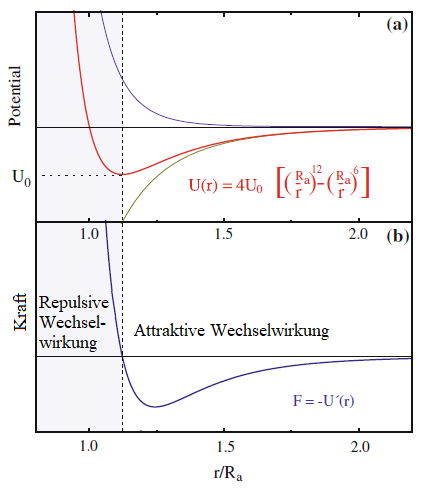
\includegraphics[width=0.5\textwidth]{Abb/LJ.png}
	\caption{Annäherung der Wechselwirkung zwischen Messspitze und Probe durch
	das Lennard-Jones-Potential (a). In (b) ist die resultierende Kraft
	$\frac{\partial U_{\text{LJ}}}{\partial r}$ dargestellt \cite[148]{AFM}.}
	\label{fig:LJ}
\end{figure}

\subsection{Messmodi}
\label{sec:Messmodi}
Zunächst werden die Messmodi in dynamische und statische Verfahren unterteilt.
Bei der dynamischen Messmodi schwingt das Cantilever nahe der Resonanzfrequenz
kontaktlos über die Probe. Wechselwirkt die Probe nun mit dem Cantilever, so verändert
sich die Cantileverschwingung geringfügig, wodurch die Topografie der Probe bestimmt
werden kann.
Bei der statischen Messmethoden wird die Messspitze über die Probe gerastert und
das Cantilever erfährt nach dem Hookeschen Gesetz eine Auslenkung. Die beiden
gängisten Messmodi sind der $\textit{Constant-Force}$ und der
$\textit{Constant-Height}$-Modus. Bei dem $\textit{Constant-Force}$-Modus wird
die Auslenkung $\Delta z$, und damit die Kraft, konstant gehalten. Dabei kann
eingestellt werden, ob die repulsive (kontaktlos) oder anziehende Kraft (Kontakt)
konstant gehalten werden soll. Um jene Kraft konstant halten zu können, wird der
Detektorstrom in eine Signalspannung $\Delta U$ transformiert, sodass mittels
eines $\textit{Feedback-loops}$ bei zu schwacher/starker Auslenkung $\Delta z$
die z-Position durch den z-Piezoelement des Cantilevers korrigiert werden kann.
So lassen sich besonders harte Proben schnell abgescannen. Weiterhin erlaubt der
$\textit{Constant-Force}$-Modus weiche Probe unbeschädigt abzumessen. Ein Nachteil
ist, dass die laterale Auflösung durch die 1-$\SI{10}{\nano\meter}$ kleine
Kontaktstelle begrenzt ist (siehe Abbildung \ref{fig:const-force}).

\begin{figure}[H]
	\centering
	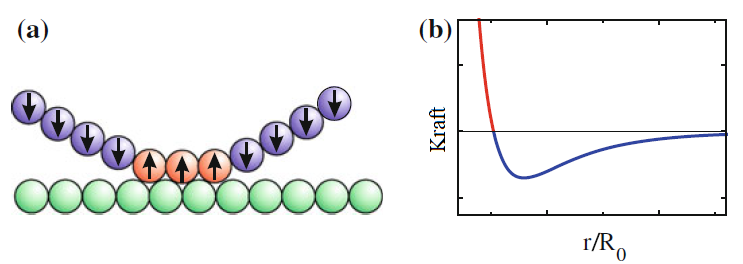
\includegraphics[width=0.8\textwidth]{Abb/const-force.png}
	\caption{Schematische Darstellung des $\textit{Constant-Force}$ Modus bezüglich
	der wirkenden Kräfte zwischen Messspitze und Probe \cite[179]{AFM}.}
	\label{fig:const-force}
\end{figure}

\noindent
Bei dem
$\textit{Constant-Height}$-Modus wird die Höhe zwischen Messspitze und Probe
konstant gehalten. So kann beispielsweise bei magnetischen Wechselwirkungen die
Probe kontaktlos abgerastert werden. Der $\textit{Constant-Height}$-Modus funktioniert
ganz ohne einen $\textit{Feedback-loops}$, wodurch das Abscannen schneller ist.
Allerdings findet der $\textit{Constant-Height}$-Modus hauptsächlich bei weitreichende
Kräfte Anwendung. Beide statische Modi sind nur für relativ ebene Proben geeignet,
denn bei starken Änderungen in der Topografie kommt es zu Artefakten.


\subsection{Kraft-Abstands-Kurve}
\label{sec:Kraft-Abstand}

Neben topografischen Karten, lässt sich auch mittels der Kraft-Abstands-Kurve das
Elastizitätsmodul $\epsilon$ einer Probe bestimmen. In Abbildung \ref{fig:Kraft-Abstand}
ist eine ideale Kraft-Abstands-Kurve dargestellt, wobei die rote/blaue Kurve die
sich annähernde/entfernende Messspitze beschreibt. Im Punkt (a) sind Probe und
Messspitze noch nicht in kontakt. Nachdem der Abstand zur Probe genügend klein
ist und die attraktive Van-der-Waals-Kraft auf die Messspitze wirkt, kommt es im
Punkt (c) zu einem $\textit{snap-to-contact}$. Im Punkt (d) wirkt sofort die repulsive
Kraft bedingt durch das Pauli-Prinzip und ein linearer Anstieg ist zu erkennen.
Sobald die Kraft auf die Probe gemindert wird, nimmt die Kraft-Abstands-Kurve,
aufgrund der starken attraktiven Adhäsionskraft, linear bis zum Punkt (f) ab.
Im Punkt (f) kommt es schließlich zum $\textit{snap-out-contact}$. In der oberen
rechten Ecke der Abbildung \ref{fig:Kraft-Abstand} sind die einzelnen Punkte (a),
(c), (d) und (f) nochmal im Lennard-Jones-Kraft-Diagramm dargestellt.

\begin{figure}[H]
	\centering
	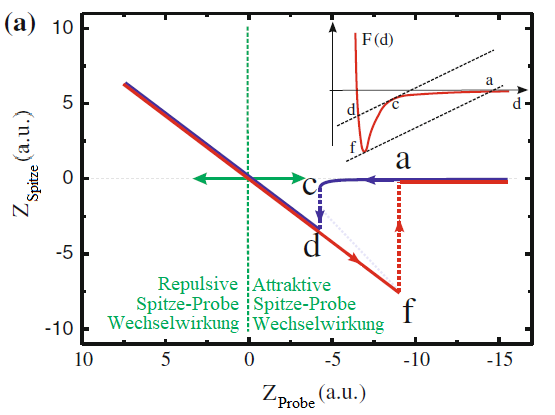
\includegraphics[width=0.7\textwidth]{Abb/Kraft-Abstands-Kurve.png}
	\caption{Ideale Kraft-Abstands-Kurve, wobei rot die annähernde und blau die
	entfernende Messspitze darstellt. (a) Messspitze noch nicht mit der Probe in
	Kontakt. (c) Die Messspitze ist genügend nah dran und es kommt zum
$\textit{snap-to-contact}$. (d) repulsive Kraft bedingt durch das Pauli-Prinzip.
	(f) Abstand genügend entfernt und es kommt zum $\textit{snap-out-contact}$
	\cite[184]{AFM}.}
	\label{fig:Kraft-Abstand}
\end{figure}
